\subsection{ADCD by Extreme Eigenvalue (ADCD-X)} \label{sec:adcd_by_extreme_eigenvalue}

The following lemma shows how to obtain a DC decomposition of a twice differential function $f(x)$.
Recall a function $f$ is convex if and only if its Hessian $H$ is positive semidefinite (denoted $H \succeq 0$), i.e., its smallest eigenvalue is non-negative.
Conversely, $f$ is concave if its largest eigenvalue is non-positive, $H \preceq 0$.
The idea behind the lemma is that $f$ can be ``made convex'' by adding another function such that the Hessian is positive semidefinite (PSD).
The added function must be convex and the difference between the altered function and the added function is the required DC decomposition.
The added function construction is based on the extreme eigenvalues of the Hessian of the function.
Note, the lemma is defined over some set $\FS$, which can be the full domain $\FD$ or a subset of it.

\begin{lemma} \label{lemma:adcd_by_extreme_eigenvalue}
Let $f(x)$ be a twice differentiable function with domain $\FD$, and let $\FS \subseteq \FD$ be a subset of the domain. 
Let $\lambda_{\min}$ and $\lambda_{\max}$ be the smallest and largest eigenvalues of the Hessian $H(x)$ of $f(x)$ where $x\in \FS$,
and define $\lambda^{-}_{\min} \coloneqq \min\{0, \lambda_{\min}\}$ and $\lambda^{+}_{\max} \coloneqq \max\{0, \lambda_{\max}\}$.

Then \eqref{eq:lemma1-convex} is a convex difference of $f(x)$ over $\FS$:
\begin{align}
\label{eq:lemma1-convex}
f(x) = \underbrace{f(x) + \frac{1}{2}\abs{\lambda^-_{\min}} \norm{x-x_0}^2 }_{\text{convex }\check{g}(x)} - \underbrace{\frac{1}{2}\abs{\lambda^-_{\min}} \norm{x-x_0}^2}_{\text{convex }\check{h}(x)}
\end{align}
and \eqref{eq:lemma1-concave} is a concave difference of $f(x)$ over $\FS$:
\begin{align}
\label{eq:lemma1-concave}
f(x) = \underbrace{ f(x) - \frac{1}{2}\lambda^{+}_{\max} \norm{x-x_0}^2 }_{\text{concave }\hat{g}(x)} - \underbrace{\frac{-1}{2}\lambda^{+}_{\max} \norm{x-x_0}^2}_{\text{concave }\hat{h}(x)}.
\end{align}
\end{lemma}


The proof of Lemma~\ref{lemma:adcd_by_extreme_eigenvalue} uses the fact that $\lambda^{-}_{\min} \leq \lambda_{\min}$ to show that Hessians of $\check{g}$ and $\check{h}$ are PSD, which implies $\check{g}$ and $\check{h}$ are convex, and similarly show that $\hat{g}$ and $\hat{h}$ are concave.
The full proof is omitted due to space limitation.


Lemma~\ref{lemma:adcd_by_extreme_eigenvalue} shows how to construct a DC decomposition if we are given the extreme eigenvalues.\footnote{An informal version of \eqref{eq:lemma1-convex} appears in~\cite{lazerson:lightweight_monitoring}, where it is used for manual analysis of specific functions rather than automatically for general function.}
Alas, finding the extreme eigenvalues of a general function, with an $x$-dependent Hessian matrix, is a difficult task~\cite{interval_matrix_branch_and_bound}.
The Hessian $H(x)$ is a function of $x$, and therefore its eigenvalues are a function of $x$.
Finding the $x$ in $\FS$ that obtains the minimal or maximal eigenvalue is not trivial.
Therefore, instead of finding the extreme eigenvalues analytically, we use numerical techniques to solve this problem.


\betterparagraph{Using Automatic Differentiation}
Using Lemma~\ref{lemma:adcd_by_extreme_eigenvalue} requires obtaining $H(x)$ and finding $x',x'' \in \FS$ that obtain $\lambda_{\min}$ and $\lambda_{\max}$.
Our key insight here is that we do not need an analytic solution for $\lambda_{\min}$ and $\lambda_{\max}$, nor a symbolic expression of $H(x)$, but rather a way to evaluate $H$ for specific points in $\FS$.
Since we are given an arbitrary $f(x)$ in the form of a short program, AD enables this automatic evaluation of $H$ in any $x \in \FS$.
By evaluating $H$ using AD at multiple points in $\FS$, and computing the extreme eigenvalues of each such Hessian, we can find the global minimum and maximum $\lambda_{\min}$ and $\lambda_{\max}$.
Instead of evaluating $H$ at random points, we define and solve an optimization problem, which is a more robust and efficient method to find these extreme values.

Another advantage of using AD is that it allows us to apply Lemma~\ref{lemma:adcd_by_extreme_eigenvalue} to functions that are not strictly twice-differentiable.
As demonstrated by the DNN with ReLU activation in \S\ref{sec:evaluation}, AD allows us to surpass this limitation as long as the function is continuous.


\betterparagraph{Finding the Eigenvalues}
After having $H(x)$ computed by AD, and the ability to evaluate it at every $x \in \FS$, we can now use it to find the extreme eigenvalues.
For this $H(x)$, we define two functions, $\lambda_{\min} \left( H(x) \right)$ and $\lambda_{\max} \left( H(x) \right)$, which yield the minimal and maximal eigenvalues of the Hessian, respectively, at a given point $x$.
We then use numerical box-constrained optimization methods (e.g., SLSQP and L-BFGS-B) to solve two optimization problems over $\FS$:
\begin{align} \label{eq:numerical_eigenvalues}
\hat{\lambda}_{\min} = \min_{x \in \FS} \lambda_{\min} \left( H(x) \right),\quad
\hat{\lambda}_{\max} = \max_{x \in \FS} \lambda_{\max} \left( H(x) \right).
\end{align}
These optimization problems are not convex, and their complexity is determined by the function $f(x)$ and its Hessian.
Therefore, there is no guarantee that the solution found by the optimization process is the global solution over $\FS$.
The numerical optimization algorithm could converge to a local minimum/maximum, a saddle point, or even not fully converge, as the number of iterations of the algorithm is limited and the problem could be ill-conditioned and require more iterations.
Hence, $\hat{\lambda}_{\min}$ and $\hat{\lambda}_{\max}$ may be different from the true $\lambda_{\min}$ and $\lambda_{\max}$.
We discuss the impact on correctness in \S\ref{sec:correctness_guarantees}.




\subsection{ADCD by Eigendecomposition (ADCD-E)} 
\label{sec:adcd_by_eigendecomposition}


DC decomposition, the representation of a function $f(x)$ as a difference of two convex/concave functions, is not unique.
Lemma~\ref{lemma:adcd_by_extreme_eigenvalue} in the previous section presented a specific DC decomposition of a function, in which the two functions are constructed using the eigenvalues of $f(x)$.
In this section, we present ADCD-E, another DC decomposition for functions with constant Hessian.
We show that this DC decomposition is superior to ADCD-X for this type of function.
The decision whether to use ADCD-E or ADCD-X is done automatically by our algorithms, as it able to automatically identify the type of the function.

The main idea behind ADCD-E is to use eigendecomposition to split the Hessian of $f(x)$ into two matrices: a positive semidefinite (PSD) matrix $H^+$ and a negative semidefinite (NSD) matrix $H^-$.
This can be done because $H$ is a constant matrix.
We obtain a convex difference of $f(x)$ using $H^-$ instead of $\lambda^{-}_{\min}$, and a concave difference using $H^+$ instead of $\lambda^{+}_{\max}$.
As before, we use automatic differentiation tools to obtain $H$, $H^-$, and $H^+$ .


\begin{lemma} \label{lemma:adcd_by_eigendecomposition}
Let $f(x)$ be a twice differentiable function with Hessian $H$ that is not a function of $x$ (i.e., it is a constant).
Let $\lambda_1 \le \lambda_2 \le ... \le \lambda_d$ be the eigenvalues of $H$, and $v_1, v_2, ..., v_d$ the corresponding eigenvectors.
The Hessian matrix $H$ is a real symmetric matrix, and can therefore be decomposed as $H=Q \Lambda Q^T$, where $Q$ is an orthonormal matrix whose columns are the eigenvectors of $H$, and $\Lambda$ is a diagonal matrix whose entries are the eigenvalues of $H$.

Let $\Lambda^-$ be a diagonal matrix whose diagonal is $[\lambda_1,...,\lambda_k, 0, ..., 0]$, and $\Lambda^+$ a diagonal matrix with diagonal $[0, ..., 0, \lambda_k+1,...,\lambda_d]$,
where $\lambda_1,...,\lambda_k$ are the negative eigenvalues and $\lambda_{k+1},...,\lambda_d$ are the non-negative eigenvalues.

Let $H^- \coloneqq Q \Lambda^- Q^T$ be the NSD part of $H$, and $H^+ \coloneqq Q \Lambda^+ Q^T$ be the PSD part.
Then a convex difference of $f(x)$ is:
\begin{align*}
f(x) = \underbrace{f(x)-\frac{1}{2} (x-x_0)^T H^- (x-x_0)}_{\text{convex }\check{g}(x)} - \underbrace{ \frac{-1}{2} (x-x_0)^T H^- (x-x_0)}_{\text{convex }\check{h}(x)},
\end{align*}
and a concave difference of $f(x)$ is:
\begin{align*}
f(x) = \underbrace{f(x)- \frac{1}{2} (x-x_0)^T H^+ (x-x_0)}_{\text{concave }\hat{g}(x)} - \underbrace{\frac{-1}{2} (x-x_0)^T H^+ (x-x_0)}_{\text{concave }\hat{h}(x)}.
\end{align*}
\end{lemma}


\begin{proof}
    Because $\Lambda = \Lambda^- + \Lambda^+$, hence $H = Q \Lambda Q^T = H^- + H^+$.
	The Hessian of $\check{g}(x)$ is $H - H^-$, which equals $H^+$.
	The matrix $H^+ = Q \Lambda^+ Q^T$ is PSD by construction since its eigenvalues are all non-negative from the definition of $\Lambda^+$.
	The Hessian of $\check{h}(x)$ is $-H^-$, which is PSD.
	Hence, $\check{g}(x)$ and $\check{h}(x)$ are convex.
    %	
	The proof of concavity for $\hat{g}(x)$ and $\hat{h}(x)$ is similar.
\end{proof}

ADCD-E can only be applied to functions that have a constant Hessian, such as inner products or quadratic forms.
For such functions, ADCD-E is superior to ADCD-X since the former results in a larger safe zone and therefore fewer local constraint violations.
Intuitively, $\check{g}_{1}$ is ``more convex'' than $\check{g}_{2}$,
where $\check{g}_{1}$ is $\check{g}$ from Lemma~\ref{lemma:adcd_by_extreme_eigenvalue} and $\check{g}_{2}$ is $\check{g}$ from Lemma~\ref{lemma:adcd_by_eigendecomposition}.

More formally, for a function with constant $H$, $H_{\check{g}_{1}} \succeq H_{\check{g}_{2}}$.
The proof follows from $H^- + \abs{\lambda^{-}_{\min}} I \succeq 0$, and therefore:
\begin{equation*}
    H_{\check{g}_{1}} = H + \abs{\lambda^{-}_{\min}} I = H^+ + H^- + \abs{\lambda^{-}_{\min}} I \succeq H^+ = H_{\check{g}_{2}},
\end{equation*}
Further, note that $\check{g}_{1}(x_0) = \check{g}_{2}(x_0)$.
This implies $\check{g}_{1} \ge \check{g}_{2}$ for every $x \in \FD$ (and similarly for $\check{h}$), which means the ADCD-X safe zone is a subset of the ADCD-E safe zone.

In summary, a safe zone violation with ADCD-E implies violation with ADCD-X but a violation with ADCD-X does not necessarily imply one with ADCD-E.
%
We can automatically detect functions with a constant Hessian by looking at the computational graph for $H(x)$ that is derived from the automatic differentiation step.

\begin{figure*}
	\centering
	\subfloat[{Admissible region is $[0.927, 2.214]$.}]{
	\label{sub_fig:sine_admissible_region}
	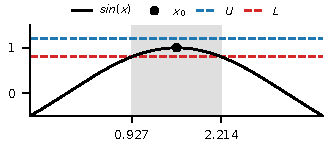
\includegraphics[width=0.32\textwidth]{figures/sine_admissible_region.pdf}
	}
	\subfloat[{Convex difference, safe zone is $[0.928, 2.203]$.}]{
	\label{sub_fig:sine_convex}
	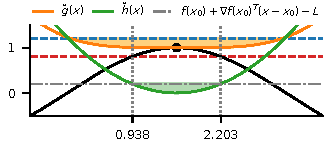
\includegraphics[width=0.32\textwidth]{figures/sine_convex_diff.pdf}
	}
	\subfloat[{Concave difference, safe zone is $[1.121, 2.202]$.}]{
	\label{sub_fig:sine_concave}
	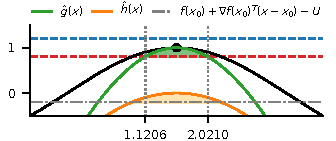
\includegraphics[width=0.32\textwidth]{figures/sine_concave_diff.pdf}
	}
	\caption{
	    ADCD local constraints for $\sin(x)$ at $x_0=\frac{\pi}{2}$.
	    Left: approximation bounds $L$ and $U$ and the resulting admissible region (gray span).
	    Middle: $\check{g},\check{h}$ of the convex difference from Lemma~\ref{lemma:adcd_by_extreme_eigenvalue}.
	    The green area shows the convex set from the upper threshold condition, and the  orange area shows the convex set of the lower threshold condition.
	    The safe zone resulting from their intersection is the area between the vertical dotted lines.
	    Right: same as middle but for $\hat{g}$ and $\hat{h}$ from the concave difference.
	}
	\label{fig:sine}
\end{figure*}




\subsection{From DC Decomposition to Constraints} 
\label{sub_sec:adcd}

After obtaining a DC decomposition of a function, the next step is to derive the ADCD local constraints.
We now show this derivation, and provide a proof that the resulting safe zone is convex, and hence guarantee correctness.

Given a convex difference $f(x) = \check{g}(x) -  \check{h}(x)$, 
we adopt the method of Lazerson et al.~\cite{lazerson:lightweight_monitoring} to derive the ADCD local constraints for $f(x)$ using the tangent plane to $\check{g}(x)$ or $\check{h}(x)$ at $x_0$:
\begin{subequations} \label{eq:convex_condition}
	\begin{align}
	&  \check{g}(x) \le \check{h}(x_0) + \nabla \check{h}(x_0)^T (x - x_0) + U, \\
	& \check{h}(x) \le \check{g}(x_0) + \nabla \check{g}(x_0)^T (x - x_0) - L.
	\end{align}
\end{subequations}
We extend this formulation for the concave difference $f(x) = \hat{g}(x) - \hat{h}(x)$, and obtain the ADCD local constraints for this difference:
\begin{subequations} \label{eq:concave_condition}
	\begin{align}
	& \hat{h}(x) \ge \hat{g}(x_0) + \nabla \hat{g}(x_0)^T (x - x_0) - U, \\
	& \hat{g}(x) \ge \hat{h}(x_0) + \nabla \hat{h}(x_0)^T (x - x_0) + L.
	\end{align}
\end{subequations}
These constraints are convex:
by opening brackets and rearranging the inequality, each inequality can be written as $\psi(x) \le C$, where $\psi$ is a convex function and $C$ is a constant, and the sets that satisfy such inequalities (sublevel sets) are convex~\cite{boyd_convex_2004}.


For the specific convex difference, in Lemma~\ref{lemma:adcd_by_extreme_eigenvalue} and in Lemma~\ref{lemma:adcd_by_eigendecomposition}, the ADCD local constraints \eqref{eq:convex_condition} can be simplified to:
\begin{align*}
\check{g}(x) \le U,\quad
\check{h}(x) \le f(x_0) + \nabla f(x_0)^T (x - x_0) - L.
\end{align*}
For the concave difference the ADCD local constraints \eqref{eq:concave_condition} are:
\begin{align*}
\hat{h}(x) \ge f(x_0) + \nabla f(x_0)^T (x - x_0) - U,\quad
\hat{g}(x) \ge L.
\end{align*}

To get the simplified form of \eqref{eq:convex_condition}, we simply note that for $\check{g},\check{h}$ in both Lemmas, $\check{h}(x_0)=0$ and $\nabla \check{h}(x_0) = 0$ and, $\check{g}(x_0) = \check{f}(x_0)$ and $\nabla \check{g}(x_0) = \nabla \check{f}(x_0)$.
Similarly, we can get the simplified form of \eqref{eq:concave_condition}.




Figure~\ref{fig:sine} shows an example of the ADCD local constraints derived for $\sin(x)$ at point $x_0=\pi/2$ according to Lemma~\ref{lemma:adcd_by_extreme_eigenvalue}.
Figure~\ref{sub_fig:sine_admissible_region} shows the admissible region, while \ref{sub_fig:sine_convex} and \ref{sub_fig:sine_concave} show the ADCD local constraints and the resulting safe zones when using convex and concave difference representations, respectively.
While both safe zones are a subset of the admissible region, they are not equivalent;
We explore this in the next subsection.




\subsection{Convex vs. Concave Difference} \label{sub_sec:convex_vs_concave_difference}

Both ADCD-X and ADCD-E provide two possible representations for a function: as a convex or as a concave difference.
In some cases, a convex difference is more efficient and results in fewer safe zone violations, while in other cases the concave difference is preferable.

Consider again the example in Figure~\ref{fig:sine} showing $\sin(x)$ with the reference point $x_0=\pi/2$.
The convex difference representation in Figure~\ref{sub_fig:sine_convex} results in a wider safe zone than the concave representation in Figure~\ref{sub_fig:sine_concave}.
Since $f$ near $x_0$ is already concave, using the concave difference results in a $\hat{g}(x)$ that is even more concave around $x_0$ than the original function $f(x)$.
However, using the convex difference obtains a convex function $\check{g}(x)$ that is "wider" than the concave function $\hat{g}(x)$, and "wider" functions tend to obtain larger safe zones.
Hence, in this case, the convex difference representation is preferable.

The curvature of $\check{g}$, $\check{h}$, $\hat{g}$, and $\hat{h}$ is determined by the eigenvalues of the Hessians of these functions, and this curvature impacts the performance of the algorithm.
Therefore, we propose the \emph{DC Heuristic} for choosing between the convex difference and concave difference, based on these eigenvalues:
if
\begin{equation*}
    \lambda_{\min} \left( H_{\check{g}}(x_0) \right) + \lambda_{\min} \left( H_{\check{h}}(x_0) \right) \le \abs{ \lambda_{\max} \left( H_{\hat{h}} (x_0) \right) + \lambda_{\max} \left( H_{\hat{g}} (x_0) \right) }
\end{equation*}
use the convex difference, otherwise use the concave difference.

The intuition behind this heuristic is to choose the representation whose two functions are less convex/concave near the reference point $x_0$.
For functions with a constant Hessian, when using ADCD-E, the heuristic condition is equivalent to $\abs{\lambda_{\min}} \le \lambda_{\max}$.

In our preliminary experiments, this heuristic reduced safe zone violations by up to 30\% when compared to using either simply the convex difference or simply the concave difference when monitoring functions such as $\sin(x)$.
